\nofiles
\documentclass[crop,tikz]{standalone}
\usepackage{amsmath}
\usepackage{scalerel}
\usepackage{tikz}
\usepackage{tikz-cd}
\usetikzlibrary{%
  matrix,%
  calc,%
  arrows%
}
\begin{document}

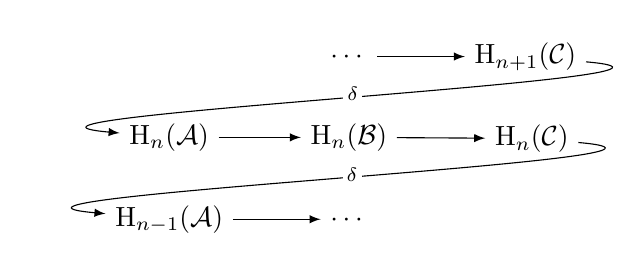
\begin{tikzpicture}[descr/.style={fill=white,inner sep=1.5pt}]
        \matrix (m) [
            matrix of nodes,
            row sep=1.5em,
            column sep=2.5em,
            text height=1.5ex, text depth=0.25ex
        ]
        {  &  & {$\cdots$} & {$\mathrm{H}_{n+1}(\mathcal C)$} \\
            & {$\mathrm{H}_n(\mathcal A)$} & {$\mathrm{H}_n(\mathcal B)$} &|[right=2.3pt, above=-5pt]| {$\mathrm{H}_n(\mathcal C)$} \\
            & {$\mathrm{H}_{n - 1}(\mathcal A)$} & {$\cdots$} & \\
        };

        \path[overlay,->, font=\scriptsize,>=latex]
        (m-1-3) edge (m-1-4)
        (m-1-4) edge[out=355,in=175] node[descr,yshift=0.3ex] {$\delta$} (m-2-2)
        (m-2-2) edge (m-2-3)
        (m-2-3) edge (m-2-4)
        (m-2-4) edge[out=355,in=175] node[descr,yshift=0.3ex,xshift=0.85ex] {$\delta$} (m-3-2)
        (m-3-2) edge (m-3-3);
\end{tikzpicture}

\end{document}